\section{Modeling HIV Transmission Dynamics - Part I}

\subsection{A first approach}
In modeling epidemics, very often, the population under consideration is assumed to be of fixed size, with births balancing deaths or migration. Such assumption is reasonable when studying endemic diseases over a large period of time and without any disease-induced deaths within the population under study. However, since HIV infections and subsequent development of AIDS have led to increased death rates in various risk groups, the population's demographic structures need to be taken into account in the modeling of the transmission dynamics of the virus.\\
The following model is largely based upon the study conducted by R.M. May and R.M. Anderson titled $\textit{The Transmission Dynamics of the Human Immunodeficiency Virus}$ published in 1988. Such study, despite being understandingly outdated in its approach to the disease (back then there was no treatment for HIV infected, for instance), is nevertheless still regarded as a good pedagogical tool to construct HIV-AIDS models using a flow-chart.\\
Consider a homosexual population of sexually-active males (age 13-65) of varying size $N(t)$ at time $t$. Assume a constant inflow of susceptible individuals at a rate $Q_{1}$ and of HIV-infectives at a rate $Q_{2}$. The population $N(t)$ is then divided in four sub-classes: 
\begin{itemize}
\item Susceptibles $S(t)$, 
\item Infected (also assumed to be infectious) $I(t)$, 
\item pre-AIDS patients $P(t)$,
\item AIDS patients $A(t)$. 
\end{itemize}
The pre-AIDS patients are individuals whose viral count is above 75 copies of virus per milliliter of blood, but have not been diagnosed with having AIDS yet. However, it is assumed that virtually all individuals in the pre-AIDS class will ultimately developed AIDS and therefore join the AIDS class.\\
All subclasses have a natural mortality rate $d$, but the total population $N(t)$ loses individuals at a higher rate from the AIDS class than from any of the others. Susceptibles sexually interact with Infected at a rate $\beta$ and with pre-AIDS patients at a rate $\beta^{\prime}$. As it is assumed that individuals in the pre-AIDS class are less sexually-active than individuals in the Infected class, then $\beta^{\prime} << \beta$. The parameter $c$ indicates the number of sexual partner for unit of time (years, in this case). It is also assumed that a fraction $\epsilon$ of infected individuals will join the pre-AIDS class (depending on the viral count) at a rate $\delta$, while another fraction (1-$\epsilon$) will join the AIDS class directly, at a rate $\delta$, as well.
Individuals in the pre-AIDS class will join the AIDS class at a rate $\alpha_{1}$, which is assumed to be much greater than the natural mortality rate $d$ of the class. Finally, individuals in the AIDS-class will have a disease-induced mortality rate of $\alpha$ and therefore a total mortality rate of ($\alpha$ + $d$). The following transfer diagram provides a helpful visualization of the the aforementioned assumptions.

\begin{center}
	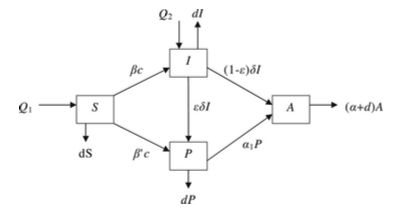
\includegraphics[scale=0.75]{HIV_Flow_Chart.png}
\end{center}

From the assumptions made, we can construct a system of Ordinary Differential Equations to describe the dynamics of the different sub-classes, as follows

\begin{align}
\frac{dS}{dt} = Q_{1} - \left(\frac{\beta cSI}{N} + \frac{\beta^{\prime} cSP}{N}\right) - dS,
\end{align}
\begin{align}
\frac{dI}{dt} = Q_{2} + \frac{\beta cSI}{N} + \frac{\beta^{\prime} cSP}{N} - (\delta + d)I,
\end{align}
\begin{align}
\frac{dP}{dt} = \epsilon\delta I - (\alpha_{1} + d)P,
\end{align}
\begin{align}
\frac{dA}{dt} = (1 - \epsilon)\delta I + \alpha_{1}P - (\alpha + d)A.
\end{align}

We see that we have a system of four differential equations with five variables, as $N(t)$ is not constant. Therefore, using the fact the total population is equal to

$$
N(t) = S(t) + I(t) + P(t) + A(t),
$$
we can rearrange the above system and write it as

\begin{align}
\frac{dN}{dt} = Q_{1} + Q_{2} -dN - \alpha A,
\end{align}
\begin{align}
\frac{dI}{dt} = Q_{2} + \frac{\beta c(N-I-P-A)I}{N} + \frac{\beta^{\prime} c(N-I-P-A)P}{N} - (\delta + d)I,
\end{align}
\begin{align}
\frac{dP}{dt} = \epsilon\delta I - (\alpha_{1} + d)P,
\end{align}
\begin{align}
\frac{dA}{dt} = (1 - \epsilon)\delta I + \alpha_{1}P - (\alpha + d)A,
\end{align}

with $N(0)>0$, $I(0)>0$, $P(0)>0$, $A(0)>0$.\\
Continuity of the right-hand side of the system and its derivative indicates that the model is well-posed for $N>0$. It is also assumed that all variables and parameters be non-negative.\\
Before proceeding in numerical simulations of the model, we first perform some stability analysis of the equilibrium.

\subsection{Equilibrium and Stability Analysis}
In our model we have a constant inflow of infected individuals at a rate $Q_{2}$, therefore the model does not exhibit a diseased-free equilibrium. However, to find all non-negative equilibria of the model, we can solve

$$
Q_{1} + Q_{2} -dN - \alpha A = 0,
$$

$$
Q_{2} + \frac{\beta c(N-I-P-A)I}{N} + \frac{\beta^{\prime} c(N-I-P-A)P}{N} - (\delta + d)I = 0,
$$

$$
\epsilon\delta I - (\alpha_{1} + d)P = 0,
$$

$$
(1 - \epsilon)\delta I + \alpha_{1}P - (\alpha + d)A = 0,
$$

which, as we shall see later, only has one non-negative solution. Such solution is the so-called $\textit{Endemic Equilibrium}$  $E^{\star} = (N^{\star},I^{\star},P^{\star},A^{\star})$, which exists as long HIV infections persist in the population, i.e. $I \neq 0$.\\

On simultaneously solving the above system of algebraic equations, we find

$$
I = \tau \xi \left(\frac{Q_{1} + Q_{2} - d N}{\alpha}\right),
$$

$$
P = \xi \left(\frac{Q_{1} + Q_{2} - d N}{\alpha}\right),
$$

$$
A = \left(\frac{Q_{1} + Q_{2} - dN}{\alpha}\right),
$$

which are all positives for $N<(Q_{1}+Q_{2})/d$.

Here

$$
\tau = \left(\frac{\alpha_{1} + d}{\epsilon \delta}\right),
$$

and

$$
\xi =  \left(\frac{(\alpha + d)}{\alpha_{1} + \frac{(1-\epsilon)}{\epsilon}(\alpha_{1}+d)}\right).
$$

Moreover,
\begin{align*}
Q_{2}N + \xi (\beta c\tau + \beta^{\prime}c) \left[N-(1+\xi+\xi\tau)\left(\frac{Q_{1}+Q_{2}-dN}{\alpha}\right)\right]\left(\frac{Q_{1}+Q_{2}-dN}{\alpha}\right)
\end{align*}
\begin{align*}
- (\delta+d) \xi\tau N \left(\frac{Q_{1}+Q_{2}-dN}{\alpha}\right) = 0.
\end{align*}

To show the existence of the endemic equilibrium $E^{\star}$, we write

\begin{align*}
F(N) = Q_{2}N + \xi (\beta c\tau + \beta^{\prime}c) \left[N-(1+\xi+\xi\tau)\left(\frac{Q_{1}+Q_{2}-dN}{\alpha}\right)\right]\left(\frac{Q_{1}+Q_{2}-dN}{\alpha}\right)
\end{align*}
\begin{align*}
- (\delta+d) \xi\tau N \left(\frac{Q_{1}+Q_{2}-dN}{\alpha}\right).
\end{align*}
From here, it is sufficient to show that the quadratic equation $F(N)$ = 0 has only one non-negative root between 0 and $(Q_{1}+Q_{2})/d$. To prove this, we see that we have

$$
F(0)=  - \xi (\beta c\tau + \beta^{\prime}c) (1+\xi+\xi\tau)\left(\frac{Q_{1}+Q_{2}-dN}{\alpha}\right)^{2} < 0
$$

and

$$
F\left(\frac{Q_{1}+Q_{2}-dN}{d}\right) = Q_{2}\left(\frac{Q_{1}+Q_{2}-dN}{d}\right) > 0.
$$

Also,

$$
F^{\prime}(N) = Q_{2} + \left[(\beta c - (\delta + d))\tau\xi + \beta^{\prime}c + \frac{2\xi d}{\alpha} (1+\tau\xi+\xi)\right] \left(\frac{Q_{1}+Q_{2}-dN}{\alpha}\right)$$
$$
- [\beta c - (\delta + d))\tau\xi + \beta^{\prime}c]\frac{dN}{\alpha}.
$$

From Calculus, we know that if $F^{\prime}(N)>0$ then the equation
$$
F(N) = 0
$$
has exactly one solution, say $N^{\star}$, between 0 and $\left(\frac{Q_{1}+Q_{2}-dN}{d}\right)$. Using $N^{\star}$ then $I^{\star}$, $P^{\star}$, $A^{\star}$ can be found, as well.\\

$\textbf{\emph{Local stability of the equilibrium point}}$\\

We can determine the nature of the local stability of the endemic equilibrium, by finding the characteristic polynomial of the following variational matrix about $E^{\star}$,

\begin{align*}
\begin{bmatrix}
-d & 0 & 0 -\alpha \\
m_{21} & -m_{22} & m_{23} & -m_{24} \\
0 & \epsilon\delta & -(\alpha_{1}+d) & 0 \\
0 & (1-\epsilon)\delta & \alpha_{1} & -(\alpha+d)
\end{bmatrix},
\end{align*}

where

$$
m_{21} = \frac{Q_{2}}{N^{\star}} + [\beta c(\delta+d)]\frac{I^{\star}}{N^{\star}} + \frac{\beta^{\prime}cP^{\star}}{N^{\star}},
$$

$$
m_{22} = \frac{Q_{2}}{I^{\star}} + \frac{\beta cI^{\star}}{N^{\star}} + \frac{\beta^{\prime} cP^{\star}}{N^{\star}} + \frac{\beta c(N^{\star}-I^{\star}-P^{\star}-A^{\star}}{N^{\star})}\left(\frac{\epsilon\delta}{\alpha_{1}+d}\right),
$$

$$
m_{23} = \frac{\beta cI^{\star}}{N^{\star}} + \frac{\beta^{\prime} cP^{\star}}{N^{\star}} + \frac{\beta^{\prime} c(I^{\star}+P^{\star}+A^{\star})}{N^{\star}} - \beta^{\prime}c,
$$

$$
m_{24} = \frac{\beta cI^{\star}}{N^{\star}} + \frac{\beta^{\prime}cP^{\star}}{N^{\star}}.
$$

The characteristic equation equation corresponding to $M(E^{\star})$ is given by
$$
f(\lambda) = \lambda^{4}+ a_{1}\lambda^{3} + a_{2}\lambda^{2} + a_{3}\lambda + a_{4} = 0,
$$
where

$$
a_{1} = 3d + \alpha + \alpha_{1} + m_{22},
$$

$$
a_{2} = (\alpha+d)(\alpha_{1}+d) + d(\alpha+\alpha_{1}+2d+m_{22}) + m_{22}(\alpha+\alpha_{1}+2d) + m_{23}\epsilon\delta+(1-\epsilon)m_{24},
$$

$$
a_{3} = d(\alpha+d)(\alpha_{1}+d) + m_{22}[(\alpha+d)(\alpha_{1}+d) + (\alpha+d)\alpha_{1}+(\alpha_{1}+d)d] + m_{24}[(1-\epsilon)\delta(\alpha_{1}+2d)]$$
$$m_{24}\epsilon\delta\alpha_{1} + m_{23}(\alpha+d)\epsilon\delta + m_{21}(1-\epsilon)\alpha\delta,
$$

$$
a_{4} = m_{22}d(\alpha+d)(\alpha_{1}+d) + m_{23}d(\alpha+d)\epsilon\delta + m_{24}d[\epsilon\delta\alpha_{1} + (1-\epsilon)\delta(\alpha_{1}+d)]$$
$$
+m_{21}\alpha\epsilon\delta\alpha_{1} + m_{21}\alpha(1-\epsilon)\delta(\alpha_{1}+d).
$$

It can readily be seen that $a_{i} > 0 $, where $i=1,2,3,4$, and $a_{1}a_{2}-a_{3}>0$, assuming that $m_{21} >0$, which implies that $\beta c \geq (\delta+d)$. Therefore, the endemic equilibrium $E^{\star}$ is locally asymptotically stable if $a_{3}(a_{1}a_{2}-a_{3}) - a_{1}^{2}a_{4} > 0$.

\subsection{Numerical Analysis and discussion}
To solve the system (2.5)-(2.8) numerically, we use the ode solver $\textit{ode45}$ in MatLab and we also find the endemic equilibrium $E^{\star}$ for the following values of parameters, taken from literature\\

$Q_{1}$=1000, $Q_{2}$=1000, $\epsilon$=0.6; d=0.02, $\alpha$=1, $\alpha_{1}$=0.5, $\beta$=0.15, $\beta^{\prime}$=0.05, c=10, $\delta$=0.4\\

with initial conditions\\
$N(0)=5000, I(0)=2000, P(0)=1000, A(0)=500$.\\
The dynamics of the population was modelled over a time interval of 30 years, following the examples found in the literature.\\

To better see how the constant immigration of both susceptible individuals and of infected people into $N(t)$ affects the dynamics of the population, we also plot our solutions for the system (2.5)-(2.8) if there there was no constant inflow of susceptibles and infected, i.e. $Q_{1}=Q_{2}=0$.

\begin{figure}[H]
	\subfigure[Model with immigration]{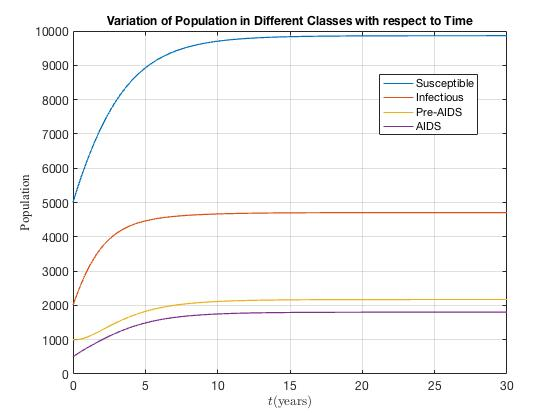
\includegraphics[scale=0.6]{hiv1.jpg}}
\end{figure}
\begin{figure}
	\subfigure[Model without immigration]{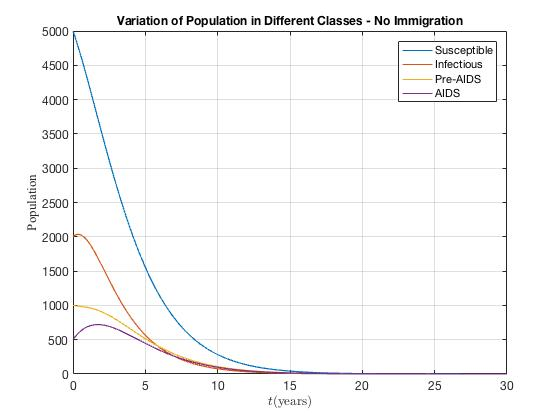
\includegraphics[scale=0.6]{hiv2.jpg}}
	\caption{Visualizing the impact of the inflow of infectious and susceptibles on the dynamics of the population}
\end{figure}

From Figure 2.1a and 2.1b, we can readily see the impact of the constant inflow of susceptible individuals and of infectious (infected) ones on the dynamics of the population.\\
In the case when there is no inflow (Fig.2.1b), the four sub-classes of individuals all decrease, ultimately exhibiting an overall exponential decay, as the total population will approach zero at around $t=15$.\\
As expected, the susceptible population decreases in size at the fastest rate, due to the fact that, without a constant inflow $Q_{1}$, the susceptibles will either die at their natural mortality rate or join either the infectious or the pre-AIDS class that will ultimately die of either AIDS or natural causes. \\
On the other hand, the initial AIDS population actually increases between $t=0$ and around $t=1$. Again, this makes sense, because this sub-class receives an input of infected individuals and pre-AIDS patients, whose total number is initially greater than the number of deaths from the AIDS-class. However, after reaching its maximum at around $t=1$, the AIDS class starts decreasing, with an interflection point at around $t=4$ and then it intersects both the infected and pre-AIDS class at $t=6$ and keeping on decreasing.\\

Conversely, in the case with a constant inflow of both susceptible and infectious individuals (Fig.2.1a), we see that all four subclasses exhibit an initial growth, with both the susceptible class and the infectious class having the faster rate of increase, as expected from the initial conditions $Q_{1}=Q_{2}=1000$. Both classes increase fast at the beginning, then the infectious class starts slowing down its growth around $t=2.5$, while the susceptible class starts to slow down after $t=4$. The infected class reaches its maximum at around $t=10$ then levels off, while the susceptible class reaches its at around $t=12$ and then levels off. \\
On the other hand, the classes of pre-AIDS patients and AIDS-patients grow more slowly compared to $I$ and $N$, increase until around $t=8$, reaching their maximum at around $t=12$ and then level off.\\

$\textbf{\emph{Equilibrium Analysis}}$\\

We focus our equilibrium analysis only to the model with a constant inflow of infected and susceptibles, i.e. $Q_{1}=Q_{2} > 0$. We use the parameters from literature and different sets of initial conditions to show that all the solutions converges to the computed equilibrium. Numerically, we find only one positive equilibrium\\

($N^{\star}$,$I^{\star}$,$P^{\star}$,$A^{\star}$) = (9863,4706,2172,1803),\\

which is the endemic equilibrium $E^{\star}$.
We compute the Jacobian matrix about this equilibrium and we find
\begin{align*}
J(E^{\star}) = \begin{bmatrix}
-0.0200 & 0  & 0  & -1 \\
0.7268  & -1.0660 & -0.7658  & -0.8258 \\
0 & 0.2400  & -0.5200 & 0 \\
0  &  0.1600 & 0.5000  & -1.0200
\end{bmatrix}.
\end{align*}

The eigenvalues are readily found to be
$\lambda_{1}=-0.3436$, $\lambda_{2}=-0.6190 + 0.2824i$, $\lambda_{3}=-0.6190 - 0.2824i$, $\lambda_{4} = -1.0443$.
Thus, we have two real negative eigenvalues and a pair of complex conjugates with negative real parts. Therefore, we have an attractive plane (connected to the real eigenvalues) and an attractive two-dimensional spiral (connected to the complex eigenvalues).\\
From the signs of the real eigenvalues and the signs of the real parts of the complex ones, we can conclude that the endemic equilibrium is locally asymptotically stable. We then plot several solutions with different initial conditions to verify this. The results are shown below.

\begin{figure}[H]
	\subfigure[S vs. P vs. A, 3D]{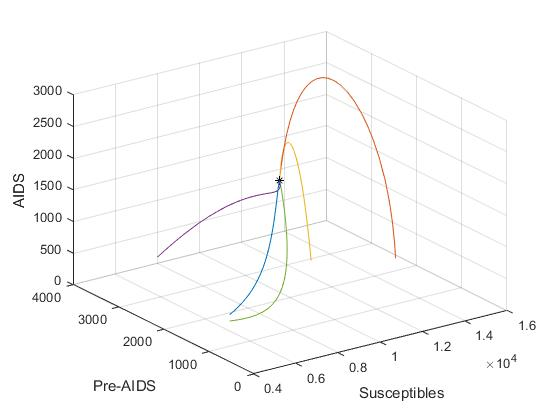
\includegraphics[scale=0.7]{hiv7.jpg}}
	\caption{Visualizing the local stability of the endemic equilibrium $E^{\star}$}
\end{figure}

So, as we can see from Fig2.2, all the solutions tend asymptotically to the endemic equilibrium, as expected from our analysis of the eigenvalues.

\subsection{Final remarks on the model}
All models are wrong, and this one makes no exception.\\
However, the model also provides some insights on how to structure an analysis of HIV transmission dynamics, giving also the opportunity to see how the study of disease was approached in the 1980's, when the epidemic erupted in the US. The model is relatively simple to solve and analyze and it is still regarded as a good pedagogical tool.\\
Nevertheless, it cannot be overstated how not including any medical treatment for HIV, while also limiting the study to a male homosexual population, represents a major flaw of this model, that cannot allow us to apply it to our time. Today we know that HIV is very much heterosexual and that drug treatment can significantly lengthen people's lives, therefore other models are required. \\
We propose one that includes drug therapy in the following section. 

\section{Modeling HIV Transmission Dynamics - Part II}
\subsection{Model of HIV/AIDS with treatment}
Over the course of many years, many treatments for HIV has been tried and implemented. Even though, up until today, there is not an effective cure for this disease, drug treatment has developed incredibly over decades and today individuals with HIV can live long and healthy life, as long as they receive treatment.\\
In fact, the process of HIV-1 pathogenesis can be slowed down by Highly Active Antiretroviral Treatment (HAART). Primarily, HAART inhibits the formation of virus particles, keeping therefore the viral load down and in turn increasing the CD4 cells count.\\
We now provide the description and analysis of a model of HIV transmission dynamics that takes into account treatment. In fact, it also considers the possibility of people receiving alternative treatment(i.e. non-HAART), as it is often the case in regions of the underdeveloped world, where access to Western-medicine-based treatment can be very problematic. The model is largely based on the research work by $\textit{Mukhtar}^{(5)}$.\\

Consider a population of size $N(t)$ at time $t$, divided into five sub-classes:
\begin{itemize}
\item \textit{S}: Susceptibles,
\item \textit{I}: Infected, but not on treatment
\item \textit{H}: Infected and on an alternative (non-HAART) treatment,
\item \textit{J}: Infected and on HAART,
\item \textit{A}: AIDS patients.
\end{itemize}

Therefore the total population $N(t)$ is
$$
N(t) = S(t) + I(t) + H(t) + J(t) + A(t).
$$

We can write down a system of differential equations to describe the population dynamics, as follows
\begin{align}
\frac{dS}{dt} = \mu k - c\beta(I+H+bJ)S - \mu S,
\end{align}
\begin{align}
\frac{dI}{dt} = (1-h)c\beta(I+H+bJ)S - (\mu+k_{1})I + \alpha(1-h_{1})J,
\end{align}
\begin{align}
\frac{dH}{dt} = hc\beta(I+H+bJ)S - (\mu+k_{1}-r)H + ah_{1}J,
\end{align}
\begin{align}
\frac{dJ}{dt} = k_{1}I + (k_{1}-r)H - (\mu+k_{2}+\alpha)J,
\end{align}
\begin{align}
\frac{dA}{dt} = k_{2}J - (\mu+d)A.
\end{align}

We now proceed to explain the parameters that appear in the above system
\begin{itemize}
\item $\mu$ is the natural mortality rate,
\item $k$ is the recruitment rate of the population,
\item $\alpha$ is the antiretroviral therapy rate,
\item $c$ is the average number of contacts between individuals per unit of time,
\item $\beta$ and b$\beta$ are the probabilities of diseased transmission per contact by an infective $I$ and by an infective $J$ respectively,
\item $k_{1}$ is the transfer rate from the asymptomatic stage to the symptomatic stage,
\item $r$ relates to the retardation effect of non-antiretroviral treatment,
\item $k_{2}$ is the transfer rate from the class $J$ to the class $A$,
\item $h$ is the fraction of the infected individuals that moves to non antiretroviral (non-ARV ) treatment,
\item $h_{1}$ is the fraction of infected individuals that have previously received ARV-treatment but now move to non-ARV treatment,
\item $d$ is the disease-induced death rate.
\end{itemize}

The variable $A$ (AIDS patients) only appears in equation (2.13) of the system (2.9)-(2.13), which means there is no interaction between the people of this class and the other four classes. That is because AIDS patients are assumed to be extremely weaken by the disease and therefore sexually inactive, so that they cannot infect others.\\
Thus, the $S$, $I$, $H$ and $J$ classes are assumed to be the active classes. The term $(I+H+bJ)S$ in equation (2.9)-(2.11) is known as an $\textit{interaction term}$. This term carries all four active classes and reflects the frequency of contact between susceptible and infected individuals.\\
For the following analysis, we can suppress equation (2.13) and our new system becomes

\begin{align}
\frac{dS}{dt} = \mu k - c\beta(I+H+bJ)S - \mu S,
\end{align}
\begin{align}
\frac{dI}{dt} = (1-h)c\beta(I+H+bJ)S - (\mu+k_{1})I + \alpha(1-h_{1})J,
\end{align}
\begin{align}
\frac{dH}{dt} = hc\beta(I+H+bJ)S - (\mu+k_{1}-r)H + ah_{1}J,
\end{align}
\begin{align}
\frac{dJ}{dt} = k_{1}I + (k_{1}-r)H - (\mu+k_{2}+\alpha)J.
\end{align}

\subsection{Equilibria and Stability}
To find the equilibria of the model (2.14)-(2.17) we have to solve

$$
\mu k - c\beta(I+H+bJ)S - \mu S = 0,
$$

$$
(1-h)c\beta(I+H+bJ)S - (\mu+k_{1})I + \alpha(1-h_{1})J = 0,
$$

$$
hc\beta(I+H+bJ)S - (\mu+k_{1}-r)H + \alpha h_{1}J = 0,
$$

$$
k_{1}I + (k_{1}-r)H - (\mu+k_{2}+\alpha)J = 0,
$$

which yields two critical points (equilibria). The first is found to be 

$$
(S_{0},I_{0},H_{0},J_{0}) = (k,0,0,0),
$$

which is the trivial critical point (disease-free equilibrium), and we indicate it as $E_{0}$. The second one is given by
\clearpage
\begin{align}
S_{1} = \frac{\mu+k_{1})\xi_{1} - \mu\alpha(1-h_{1})r}{c\beta[\xi_{3}+hr(\mu+k_{2}-b\mu)+\alpha h_{1}r]},
\end{align}

\begin{align}
I_{1} = \frac{\mu k [(1-h)\xi_{1} + (k_{1}-r)\alpha(1-h_{1})]}{(\mu+k_{1})\xi_{1} - \mu\alpha(1-h_{1})r},
\end{align}

\begin{align}
H_{1} = \frac{\mu k[h\xi_{2}+k_{1}\alpha h_{1}]}{(\mu+k_{1})\xi_{1} - \mu\alpha(1-h_{1})r},
\end{align}

\begin{align}
J_{1} = \frac{\mu k[(\mu+k_{1}-r)k_{1} - h\mu r]}{(\mu+k_{1})\xi_{1} - \mu\alpha(1-h_{1})r},
\end{align}

which is the endemic equilibrium ($E_{1}$), where

\begin{align*}
\xi_{1} = (\mu+k_{1}-r)(\mu + k_{2} +\alpha) - \alpha(k_{1}-r),
\end{align*}
\begin{align*}
\xi_{2} = (\mu+k_{1})(\mu+k_{2}+\alpha)-\alpha k_{1},
\end{align*}
\begin{align*}
\xi_{3} = (\mu+k_{1}-r)(\mu+k_{2}+\alpha+bk_{1}).
\end{align*}

To study the nature of the equilibria we first need to compute the $\textit{basic reproduction number}$ $R_{0}$, which is defined as the expected number of secondary infections arising from a single individual during his/her infectious period, in a population of susceptibles. This parameter plays an important role in the control and eradication of epidemics. \\
If $R_{0}<1$, then, on average, an infected individual produces less than one newly infected individual and the epidemic dies out. On the other hand, if $R_{0} >1$, then each infected individual produces, on average, more than one newly infected individual and, therefore, the epidemic spreads out into the population. In such regard, $R_{0}$ is often considered the threshold quantity that indicates if an infection will invade and persist a population. 
For the system (2.14)-(2.17) the basic reproduction number is found to be

\begin{align}
R_{0} = \frac{c\beta k[\xi_{3}+hr(\mu+k_{?}-b\mu)+\alpha h_{1}r]}{(\mu+k_{1})\xi_{1} -\mu\alpha(1-h_{1})r}.
\end{align}
From literature, we know that the disease-free equilibrium $E_{0}$ is locally asymptotically stable if $R_{0} < 1$ and unstable otherwise. Whereas, the endemic equilibrium $E_{1}$ is stable if $R_{0} > 1$ and unstable if $R_{0} < 1$.\\
In the following section we perform some numerical analysis with different values of parameters to simulate both the case when $R_{0} < 1$ and $R_{0}>1$.

\section{Numerical Simulations}
For the first simulation we use the following variables for the parameters, taken from literature
\\

$k$=120, $\beta$=0.000035, $b$ = 0.3, $\mu$=0.02, $c$=3, $k_{1}$=0.01, $k_{2}$=0.02 $\alpha$=0.01, $h$=0.01, $r$=0.001 and $h$=0.02.\\

By plugging in those values into (2.22) we obtain
$$
R_{0} = 0.45 < 1,
$$
which means that the epidemic should die out for the given values of the parameters. We now plot our results

\begin{figure}[H]
	{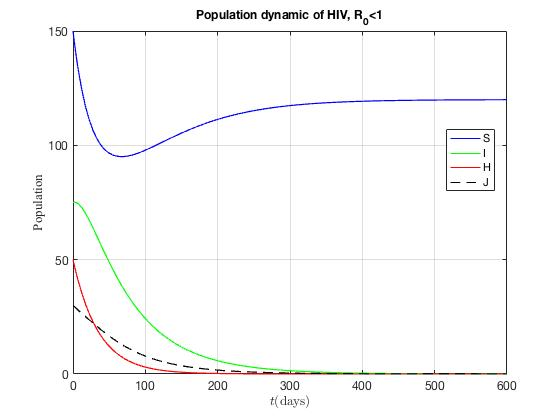
\includegraphics[scale=0.7]{hiv_art.jpg}}
	\caption{Simulation for $R_{0} < 1$}
\end{figure}

Thus, we see from figure 2.3 that, for a basic reproduction number that is less than unity, the population of susceptibles $S$ decreases at first and then starts increasing back at around $t=95$ as the infected population of all the other classes, regardless of treatment, starts to quickly approaching zero. The susceptible population seems to be levelling off at around $t=400$, when the classes $I$, $J$ and $H$ all reaches zero.\\
From an equilibrium point perspective, this makes sense as we have a value for $R_{0}$ that is less then 1; therefore, the solutions will tend to the locally asymptotically stable disease-free equilibrium, and the disease will eventually die out.\\

Now we simulate the case for which the basic reproduction number is greater than unity. For this numerical simulation we use the parameters (from literature)\\

$k$=120, $\beta$=0.0005, $b$ = 0.3, $\mu$=0.02, $c$=3, $k_{1}$=0.01, $k_{2}$=0.02 $\alpha$=0.01, $h$=0.01, $r$=0.001 and $h$=0.02.\\

Plugging those values back into (2.22) yields

$$
R_{0} = 3.8 > 1,
$$
which means that the epidemic should invade the population and persist. We now plot our results

\begin{figure}[H]
	{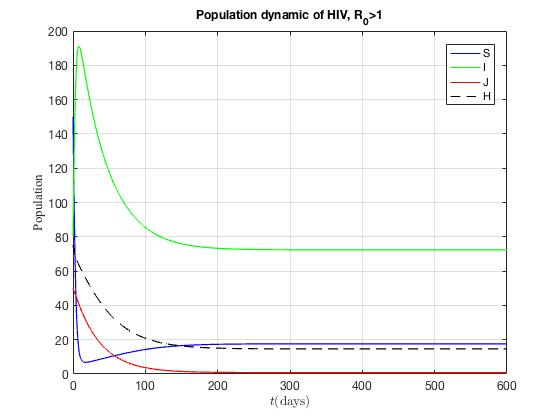
\includegraphics[scale=0.7]{hiv_art2.jpg}}
	\caption{Simulation for $R_{0} > 1$}
\end{figure}

Thus, we see that the class of susceptible individuals $S$ rapidly decreases up until $t=20$ when it reaches its minimum, then starts increasing asymptotically towards the endemic equilibrium as time goes on. On the other hand, the class of infected individuals with no treatment $I$, rapidly increases at the beginning, almost mirroring the class $S$, up until around $t=20$ when it reaches its maximum then starts to decrease until around $t=200$, when it levels off. The classes of infected with ARV treatment $J$ and infected with no ARV treatment $H$ exhibit an exponential decay from the beginning.\\
This is in accordance with the expected behavior from our equilibrium analysis, as we see that for a basic reproduction number $R_{0}$ greater than unity, the disease spreads into the population and all solution tend asymptotically to the endemic equilibrium.

\subsection{Final remarks on the model}
So we have seen that this model takes into account antiretroviral treatment as long as alternative forms of treatments in the modeling of the dynamics of a population. In this regard, it represents a step forward compared to the model analysed in section 2.1.1, but it can readily be seen how this model has built upon some of the insights provided by the earlier model.\\
Moreover, including the possibility of no-ARV treatment is an extremely realistic feature to be added to the model, as many individuals across the world, especially in underdeveloped countries, do not have access to Western-medicine-based treatments.